\documentclass[10pt]{beamer}
\usetheme{metropolis}
\usepackage{appendixnumberbeamer}
\usepackage{booktabs}
\usepackage{graphicx}
\usepackage[ruled,vlined]{algorithm2e}
\usepackage{algorithmic} 
\usepackage[scale=2]{ccicons}
\usepackage{epstopdf}
\usepackage{hyperref}
\usepackage{float}


\usepackage{pgfplots}
\usepgfplotslibrary{dateplot}

\usepackage{xspace}
\newcommand{\themename}{\textbf{\textsc{metropolis}}\xspace}

\title{GPU Accelerated Support Vector Machines via Quadratic Programming}
\date{\today}
\author{Armaan Kohli}
\institute{The Cooper Union \\ ECE453}

\begin{document}

\maketitle

\begin{frame}[fragile]{Objective}
Solve classification problems quickly
 \begin{itemize}
		\item Support Vector Machines
     	\item ADMM Algorithm
     	\item CPU and GPU Implementations
     	\item Results
	\end{itemize}
Paper from Oxford Control Group (part of \texttt{osqp}) 

GPU Acceleration of ADMM for Large-Scale Quadratic Programming \cite{cuosqp}

Michel Schubiger, Goran Banjac, and John Lygeros - 2019

  
\end{frame}

%\section{SVM}

\begin{frame}[fragile]{Support Vector Machine}
%\begin{equation}
%\{ x: f(x) = x^T\beta + 1 = 0 \}
%\end{equation}
\begin{figure}
    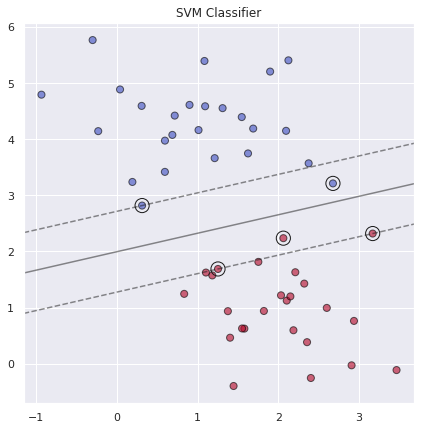
\includegraphics[scale=.4]{./media/svm.png}
    \caption{Cartoon of an SVM classification problem}
  \end{figure}
\end{frame}

\begin{frame}[fragile]{Support Vector Machine}
We can write the SVM problem as one that relies on convex optimization, specifically \textit{quadratic programming}
\begin{equation}
\{ x: f(x) = x^T\beta + 1 = 0 \}
\end{equation}
\end{frame}

\begin{frame}[fragile]{Support Vector Machine}
We can write the SVM problem as one that relies on convex optimization, specifically \textit{quadratic programming} \cite{stat}

\begin{equation}
L_P = \frac{1}{2}||\beta||^2 + C \sum_{i=1}^{N} \xi_i - \sum_{i=1}^{N}
 \alpha_i \left[ y_i \left( x_i ^T \beta +1 \right) - (1-\xi_i)\right] - \sum_{i=1}^{N} \mu_i \xi_i
\end{equation}

\begin{equation}
L_D = \sum_{i=1}^{N} \alpha_i - \frac{1}{2}\sum_{i=1}^{N} \sum_{j=1}^{N} \alpha_i \alpha_j y_i y_j x_i^T x_j
\end{equation}

\begin{equation}
\alpha_i [y_i (x_i^T \beta + 1) - (1-\xi_i)] = 0
\end{equation}

\begin{equation}
mu_i\xi_i = 0
\end{equation}

\begin{equation}
y_i(x_i^T\beta + 1) - (1-\xi_i) \geq 0
\end{equation}
This allows us to solve the SVM problem with an algorithm called ADMM
\end{frame}

%\section{ADMM}

\begin{frame}[fragile]{ADMM}
Alternating Direction Method of Multipliers
 \begin{itemize}

\item A technique to minimize convex functions
\item Intuition: Try to minimize a convex function by alternatively minimize Lagrangian in different directions 
\end{itemize}
\end{frame}

\begin{frame}[fragile]{ADMM}
\begin{algorithm}[H]
\SetKwInOut{Input}{input}\SetKwInOut{Output}{output} 
\SetAlgoLined
\textit{given:}
 $x^0, z^0, y^0 \; \textit{and parameters} \;\rho >0, \; \sigma >0, \; \alpha \in [0,2]$
 \\ \While{\textit{not terminated}}{
 ${(\tilde{x}^{k+1}, v^{k+1}) \leftarrow \begin{bmatrix}
P+\sigma I & A^T\\
A & -\rho^{-1}I  
\end{bmatrix}}
\begin{bmatrix}
\tilde{x}^{k+1}\\
v^{k+1}
\end{bmatrix}
= \begin{bmatrix}
\sigma x^k - q\\
z^k - \rho^{-1}y^k
\end{bmatrix}
$
\\
$\tilde{z}^{k+1} \leftarrow z^k + \rho^{-1}(v^{k+1} - y^k)$\\
$x^{k+1} \leftarrow \alpha\tilde{x}^{k+1} + (1-\alpha)x^k$ \\
$z^{k+1} \leftarrow \prod \left(\alpha\tilde{z}^{k+1}+(1-\alpha)z^k + \rho^{-1}y^k \right)$ \\
$y^{k+1} \leftarrow y^k + \rho(\alpha \tilde{z}^{k+1} + (1-\alpha)z^k - z^{k+1}$
 } \caption{ADMM algorithm as presented in \cite{osqp}}
\end{algorithm}
\end{frame}

\begin{frame}[fragile]{ADMM}
Issue: solving this linear system is challenging
\begin{equation}
\begin{bmatrix}
P+\sigma I & A^T\\
A & -\rho^{-1}I  
\end{bmatrix}
\begin{bmatrix}
\tilde{x}^{k+1}\\
v^{k+1}
\end{bmatrix}
= \begin{bmatrix}
\sigma x^k - q\\
z^k - \rho^{-1}y^k
\end{bmatrix}
\end{equation}
\end{frame}

\begin{frame}[fragile]{ADMM}
Issue: solving this linear system is challenging
\begin{equation}
\begin{bmatrix}
P+\sigma I & A^T\\
A & -\rho^{-1}I  
\end{bmatrix}
\begin{bmatrix}
\tilde{x}^{k+1}\\
v^{k+1}
\end{bmatrix}
= \begin{bmatrix}
\sigma x^k - q\\
z^k - \rho^{-1}y^k
\end{bmatrix}
\end{equation}
\begin{itemize}
\item Use LDL Factorization
\item Use Preconditioned Conjugate Gradient (PCG)
\end{itemize}
\end{frame}


\begin{frame}[fragile]{PCG}

\begin{algorithm}[H]
\SetKwInOut{Input}{input}\SetKwInOut{Output}{output} 
\SetAlgoLined
\textit{initialise:}
 $r^0 = Kx^0 -b, \; y^0 = M^{-1}r^0, \; p^0 = -y^0, \; k = 0 $
 \\ \While{$||r^k|| > \epsilon||b||$}{
$\alpha^k \leftarrow - \frac{\left(r^k\right)^Ty^k}{\left(p^k\right)^TKp^k} $\\
$x^{k+1} \leftarrow x^k + \alpha^k p^k$\\
$r^{k+1} \leftarrow r^k + \alpha^k K p^k$\\
$y^{k+1} \leftarrow M^{-1}r^{k+1}$\\
$\beta^{k+1} \leftarrow - \frac{\left(r^{k+1}\right)^Ty^{k+1}}{\left(r^k\right)^Ty^k} $\\
$p^{k+1} \leftarrow -y^{k+1} + \beta^{k+1}p^k$\\
$k \leftarrow k + 1 $
 } \caption{PCG algorithm as presented in \cite{cuosqp}}
\end{algorithm}


\end{frame}

\begin{frame}[fragile]{GPU Optimizations}
\begin{itemize}
\item matrix representation - CSR
\item \texttt{cuBLAS}
\item \texttt{cuSPARSE}
\end{itemize}
\end{frame}


\begin{frame}[fragile]{Results}
  \begin{figure}
    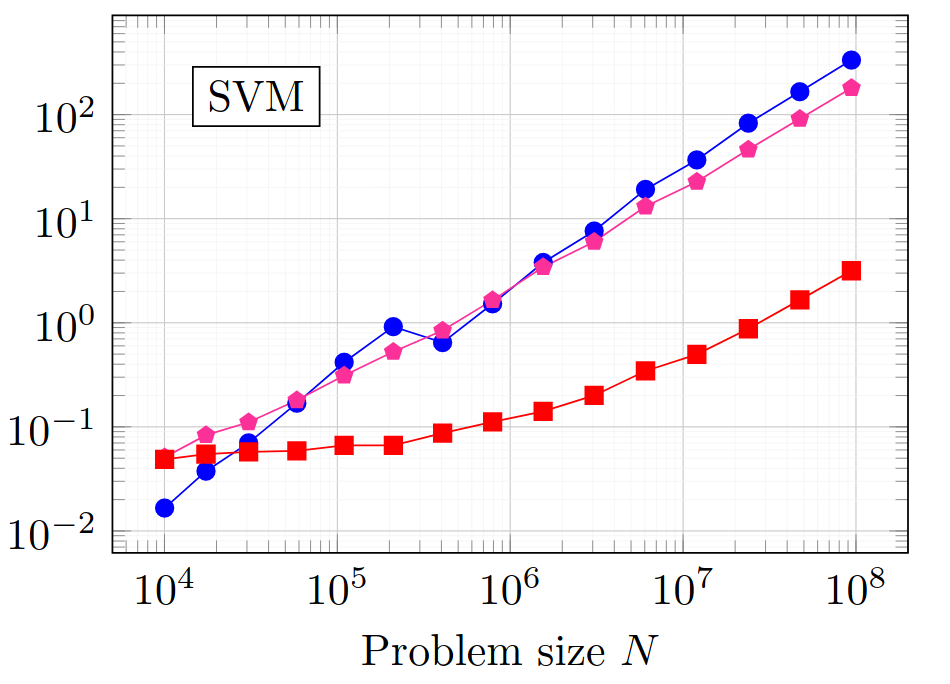
\includegraphics[width=.5\textwidth]{./media/cuosqp_results.png}%
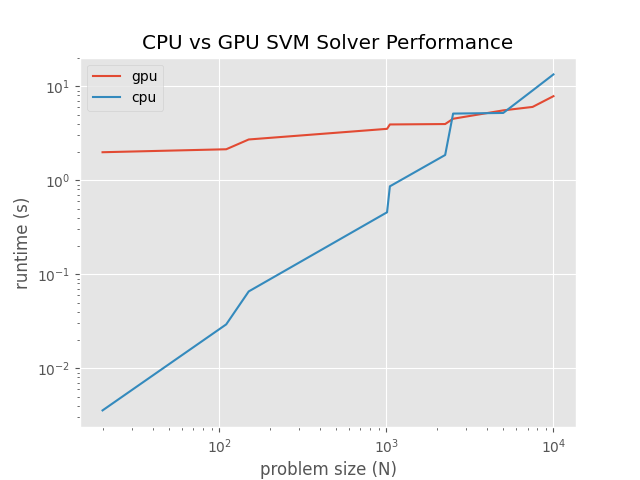
\includegraphics[width=.5\textwidth]{./media/results.png}
  \end{figure}
\end{frame}



\begin{frame}[fragile]{References}

  \bibliography{bib}
  \bibliographystyle{abbrv}

\end{frame}

\end{document}
